\documentclass[../rapport.tex]{subfiles}

\begin{document}
\begin{enumerate}
	\item{Autoriser les virements}\\
		\begin{figure}[h]
			\centering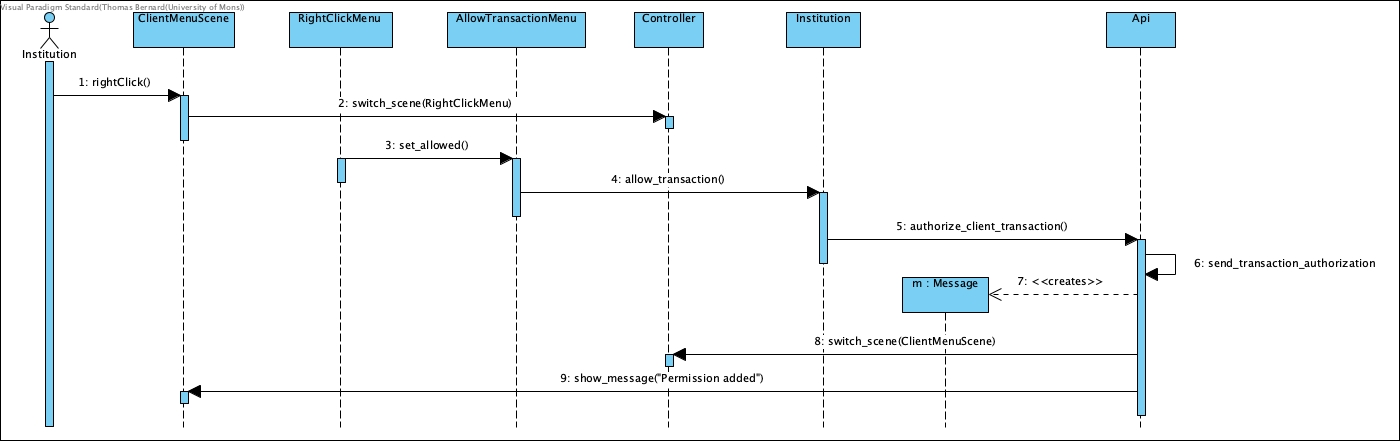
\includegraphics[scale=0.25]{ressources/photos_diagrammes/app2/sequences2/autoriserVirement.jpg}
			\caption{Autoriser les virements}
		\end{figure}\\
Ce diagramme décrit la procédure qu'effectue un employé d'une institution afin d'activer les virements pour un client de l'institution.
La procédure est relativement simple, une fois que l'employée a cliqué sur le bouton d'activation, une requête est envoyée à l'api afin d'activer la fonctionnalité dans la base de données.
\newpage
	\item{Cloturer un produit financier}\\
		\begin{figure}[h]
			\centering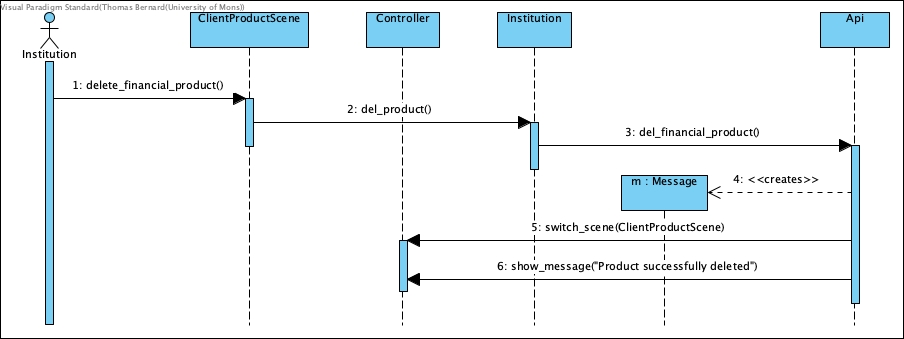
\includegraphics[scale=0.25]{ressources/photos_diagrammes/app2/sequences2/cloturerProduitFinancier.jpg}
			\caption{Cloturer un produit financier}
		\end{figure}\\
Lorqu'un employé d'institution cloture un produit financier d'un client, une requète est envoyée au serveur afin de désactiver le produit dans la base de donnée. Le produit n'est pas réellement définitivement supprimé.
\newpage
	\item{Consulter la liste des produits financiers}\\
		\begin{figure}[h]
			\centering\includegraphics[scale=0.25]{ressources/photos_diagrammes/app2/sequences2/consulterListeproduits.jpg}
			\caption{Consulter la liste des produit financiers}
		\end{figure}\\
Après avoir sélectionner un client, un employé d'une institution financière peut consulter la liste des produits de son client. Une première requète à l'api récupèrera la liste des clients et une deuxième requête s'occupera de récupérer les produits d'un client sélectionné.
\newpage
	\item{Supprimer un client}
		\begin{figure}[h]
			\centering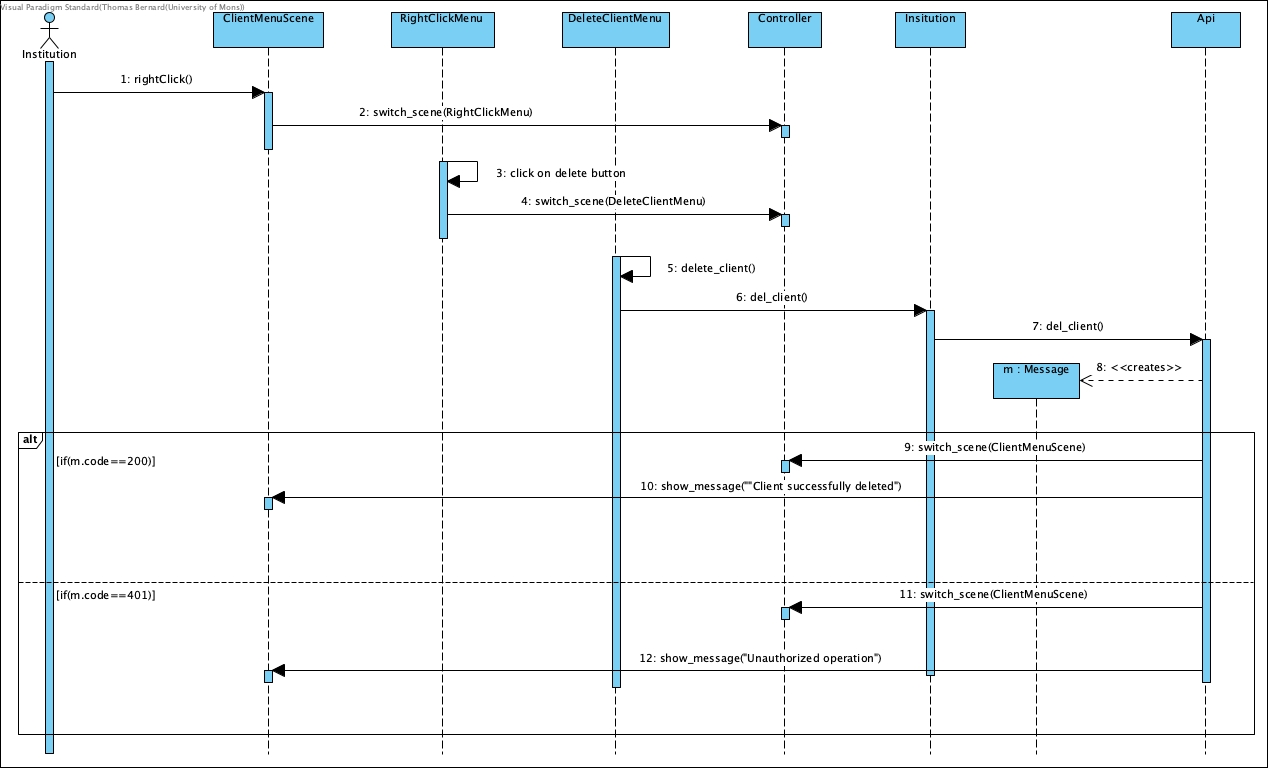
\includegraphics[scale=0.25]{ressources/photos_diagrammes/app2/sequences2/supprimerClient.jpg}
			\caption{Supprimer un client de l'institution}
		\end{figure}\\
Un employé d'une institution peut choisir de supprimer un client via le menu de suppression de clients. Une requète est alors envoyé à l'api qui confirmera ensuite l'opération en indiquant si elle a réussi ou non.
\end{enumerate}
\newpage
\end{document}
